\section{CAPÍTULO IV: METODOLOGÍA}\label{sec:methodology}

En este capítulo, se describirá la metodología utilizada para conseguir cumplir los objetivos establecidos. 

Se comenzará por discutir el diseño de la investigación y los tipos de variables que serán utilizados a la hora de realizar el estudio. Luego se describirá el enfoque aportado para el preprocesamiento de datos, incluida la limpieza de datos y la selección de características.

Finalmente, se describirán los algoritmos de aprendizaje automático utilizados para el estudio y clasificación de pacientes. 

\subsection{Diseño de Investigación}

Se ha utilizado un enfoque de investigación cuantitativa para examinar la progresión temporal de la bronquiolitis en pacientes pediátricos. Como se ha mencionado anteriormente se van a realizar $2$ estudios diferentes con distinto enfoque:

\begin{itemize}
    \item El primer estudio, \textit{Estudio 1}, como se ha tratado anteriormente en la Sección~\ref{sec:metodologias_exclusion_pacientes} de selección de pacientes válidos para los distintos estudios, se va a centrar en el estudio de todos los pacientes pediátricos considerando las primeras $24$ horas desde el ingreso. En este caso se valorará de manera general la evolución de los pacientes y diferencias entre aquellos que se les ha intervenido con OAF y los que no. En este estudio simplemente se tendrán en consideración las variables \textit{Series Temporales} referenciadas en la tabla~\ref{tabla:variables_estudio} y se realizará un estudio descriptivo de las mismas.
    \item  En el segundo estudio, \textit{Estudio 2}, se valorará la evolución de los pacientes que han necesitado OAF y se comparará con los que no han necesitado OAF para así poder generar un modelo que permita predecir si un paciente va a necesitar OAF o no en las siguientes próximas horas. Es este estudio se pretenderá realizar un modelo que permita prever la necesidad de OAF en las 8 h de ingreso. ad de OAF en las horas siguientes de las 
\end{itemize}

Se utilizarán aquellas variables que se han definido anteriormente en la Sección~\ref{sec:tiposdevariables} y en concreto de aquellas recogidas en la Tabla~\ref{tabla:variables_estudio}:

\begin{itemize}
    \item Descriptivas dentro del \textit{scope} del estudio.
    \item Temporales en $3$ Intervalos dentro del \textit{scope}.
    \item Series Temporales.
\end{itemize}

Las variables utilizadas e el \textit{Estudio 2} será menos que las usadas en el \textit{Estudio 1}

ha partido de 47 variables descriptivas y de 2 variables que muestran la evolución temporal de los pacientes durante las primeras 24 h de ingreso y que han sido tratadas en el presente trabajo como series temporales. 


Explicación de los distintos Estudios:


En el caso del Estudio 2:

Idealmente 

Idealmente se ha planteado que al tener 3 momentos de valoración; en las $8$ primeras horas, entre las $8$ y $16$ horas siguientes y entre las $16$ y $24$ últimas horas, se realicen $3$ modelos distintos de clasificación para los diferentes momentos de valoración y que estos modelos permitan valorar la evolución del paciente, es decir si va a necesitar OAF o no va a necesitarla al final de estos intervalos. Es decir, una vez pasadas las $8$ primeas horas se pretende valorar si el paciente va a necesitar OAF en las próximas $8$ horas y así sucesivamente. 

De cara a plantear esta metodología para este estudio existe el factor limitante de la muestra de pacientes con la que se trabaja, dónde la mayoría de pacientes no sufren OAF y por tanto no se puede realizar un estudio de este tipo dónde se divide por intervalos a la muestra de pacientes que sufren OAF. A continuación se muestra en relación al \textit{Estudio 1} cómo se distribuyen los pacientes que han necesitado OAF:

En este estudio este planteamiento se muestra limitado puesto que más de la mitad de pacientes que se han considerado válidos para el estudio (según el criterio valid\_patient\_2 adoptado en el apartado ***) que necesitan OAF la requieren al ingreso o en las primeras 8 horas (De los 16 pacientes válidos que presentan deterioro 10 pacientes; 5 al ingreso y 5 antes de las 8 primeras horas). Esto supondría eliminar de la ecuación estos 10 pacientes y solo tener en cuenta a los 6 restantes para valorar las 8 primeras horas y solo a 2 para valorar las 16 primeras.

\begin{figure}[H]
    \centering
    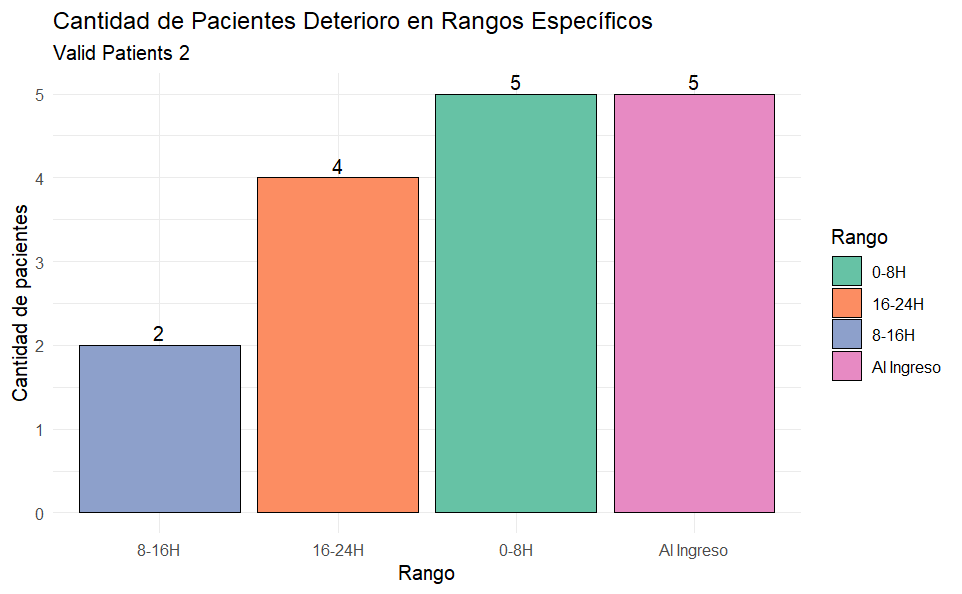
\includegraphics[scale = 1]{./img/bar-deterioro-valid-2.png}
    \caption{Cantidad de Pacientes Deterioro en Rangos Específicos de Tiempo considerando solo los pacientes sgún criterio valid\_patient\_2}
    \label{fig:bar-deterioro-valid-2}
\end{figure}

Se va a separar entre pacientes que han necesitado OAF al ingreso y los que no.

A continuación se muestran en rojo aquellos pacientes que a pesar de haberles suministrado OAF han necesitado ser trasladados a UCIP.

En contraposición se muestran en verde aquellos pacientes que han necesitado OAF pero no han necesitado ser trasladados a UCIP. 



Ningún paciente cómo ya se ha visto ha necesitado traslado a UCIP sin haber necesitado OAF previamente.

